\documentclass[10pt]{article}

\usepackage{amsmath}
\usepackage[margin=1in]{geometry}
\usepackage{graphicx}
\usepackage{url}
\usepackage{setspace}
\usepackage{biblatex} % A library for bibliography commands.

\doublespacing

\setlength{\oddsidemargin}{0.25in}
\setlength{\textwidth}{6.5in}
\setlength{\topmargin}{-0.5in}
\setlength{\textheight}{8.5in}


\title{ECS 289F - Network Theory and Applications\\ Communities for A Better Yelp }
\author{Leyuan Wang and Edmund Yan}

\bibliography{report}

\begin{document}
\maketitle
\begin{abstract}
Yelp.com, has become a cornerstone of the internet we know today, yet it lacks the basic features of personalization.  In this paper, we implement a new method for calculating business ratings that is based on community detection.  We place users into communities of like-minded people, and see if they provide a better predictor of what a user will rate a business.  It turns out though, that counter to our original thoughts, the consensus of those in your community are no better predictors than the consensus of the rest of the population and in fact, can be worse because of the small sample size.
\end{abstract}


\section{Introduction}

Yelp is a website that provides business listings and allows customers to write reviews for ratings.  It has become an immensely popular website, climbing to being the 28th most popular website in the United States \cite{AlexaYelp}.  Part of its success can be attributed to their focus on building a great internal community of "Yelpers" through combining elements of social networking with friends and incentivizing users with badges and "Yelp Elite" status, an invite-only exclusive club.  Yelpers rate businesses by giving them stars in the range of 1 to 5 and the business has an average rating that is shown to users.

We think we can do a better job at providing a rating to users than just an average.  Yelp has accumulated a wealth of information on businesses, users, and activities between them, yet they use none of that information in providing better results for users.  Our approach will be to use community detection methods to analyze the social graph of friends and also the bipartite network of users to businesses to give a more personalized result.  Our hypothesis is that people in your community know what you like more than the rest of the population.  So if all of your friends are are raving about a particular restaurant, we think this will make it more likely that you will enjoy the restaurant as well.  Additionally, by analyzing the bipartite network, we can potentially unveil interesting pairings that would otherwise not be apparent.  Users who frequently visit the same restaurants as a particular user, shows a starking similarity in their food preferences.  We think that by categorizing users to communities, we can give more weight to the ratings from other users in the same community and thus provide a more accurate business rating.

\section{Previous Work}

TODO
TODO: Do we need to rewrite this since we use much different community detection algorithms?

For this project, were going to be focusing on two main aspects of the Yelp data. First will be
the social network of Yelp users and their friends. The second will be the bipartite network
connecting users and businesses, where edges are reviews by that user to the business
in question. After detecting communities in this two graphs, we are going to personalize
the business stars according to which community the user is in. For the first part, we found different models
for community detection. In \cite{fortunato2010community}, they give a thorough exposition of community detection methods. In \cite{newman2004finding}, several community detection methods like natural divisions of network nodes
into densely connected subgroups, are studied. The algorithm involves iterative removal
of edges from the network, and the connected components of the remaining network are the communities. For the second part, In \cite{liu2009community}, they proposed a fast algorithm called LP\&BRIM for community detection in large-scale bipartite networks. It is based on a joint strategy of two developed algorithms -- label propagation (LP), a very fast community detection algorithm, and BRIM, an algorithm for generating better community structure by recursively inducing divisions between the two types of nodes in bipartite networks. And this algorithm successfully finds meaningful community structures in large-scale bipartite networks in reasonable time limit. But there's a limit of time to implement their algorithm. If we evaluate the user directly instead of the reviews she wrote, the bipartite structure between users and businesses will be similar to the hub and authority set-up in HITS.



\section{Data}

Yelp has provided an academic dataset that contains a sample of their data from Phoenix, Arizona.  This dataset has 15,185 total businesses, 335,022 reviews, 70,817 users, and a slew of other information that we don't track in this study.  We construct two graphs from this data.  The first is a social network of users and their friends, with the 70,817 nodes, 151,516 edges and an average degree of 4.279.  As seen in the degree distribution of Figure~\ref{fig:social_degree}, the graph is scale-free and follows a power law distribution.

\begin{figure}[ht]
  \centering
    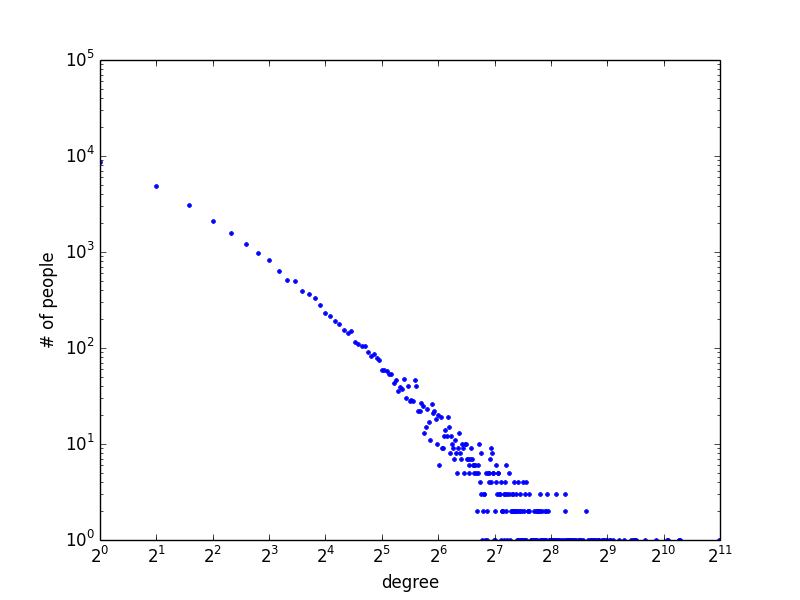
\includegraphics[width=0.5\textwidth]{soc_degree_distribution.png}
  \caption{Degree distribution of social network}
  \label{fig:social_degree}
\end{figure}


The second is a bipartite graph of users and businesses, with an edge connecting between them signifying that user has rated the business.  The weight on the edge is the 'star' attribute associated with that rating.  As said above, there were 70,817 users, with an average degree of 4.560, and 15,579 businesses, with an average degree of 20.727. Figures~\ref{fig:bipartite_degree_user}/\ref{fig:bipartite_degree_biz} shows the distribution for both types of nodes.

\begin{figure}[ht]
\minipage{0.49\textwidth}
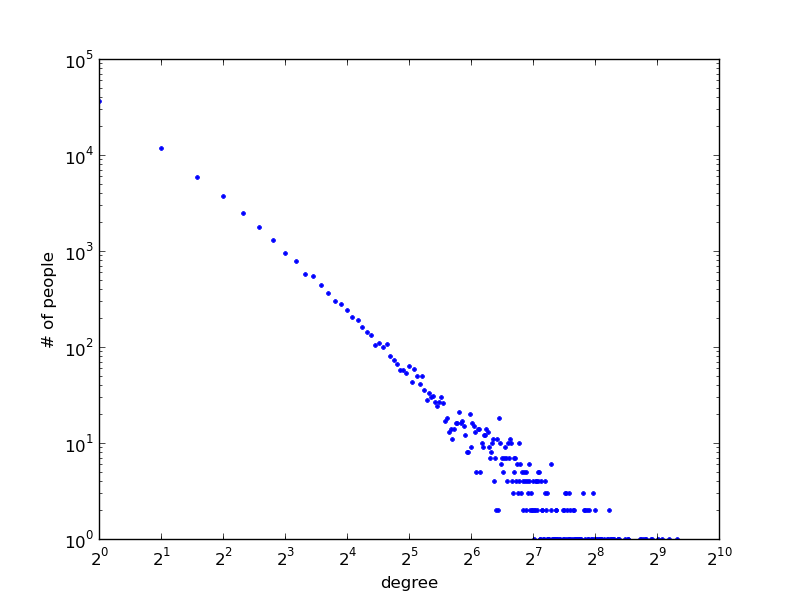
\includegraphics[scale=.4]{user_degree_distribution.png} 
\caption{Degree Distribution of Users}
\label{fig:bipartite_degree_user}
\endminipage\hfill
\minipage{0.49\textwidth}
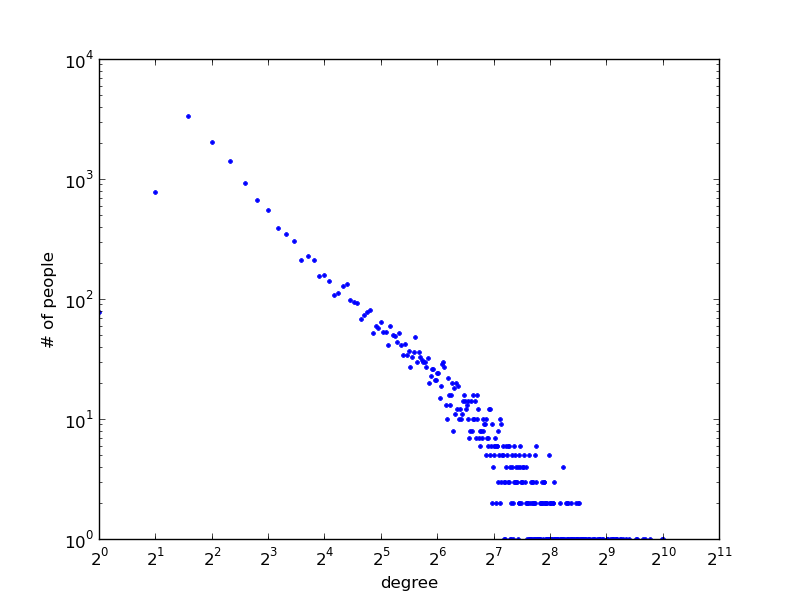
\includegraphics[scale=.4]{biz_degree_distribution.png}
\caption{Degree Distribution of Businesses}
\label{fig:bipartite_degree_biz}
\endminipage\hfill
\end{figure}

We actually use a shrunken version of both graphs because of computational restrictions, which we will discuss in the next section.

\section{Methods}

\subsection{Bipartite Graph}

To do community detection on the bipartite graph, we first do a one-mode projection onto the Users.  Simply, if user A and user B both rate a business X, we add an edge between A and B in the projected graph; the new graph only has user nodes.  This algorithm leads to an immensely dense graph, with a projection of the original bipartite graph having 2,945,687 edges with only 70,817 nodes.  Community detection algorithms on this graph were both time consuming and produced bad results.  We thus add two methods to shrink this projection into a more usable graph.  The first is a "shrink" operation that removed nodes (both users and businesses) in the bipartite graph that have a degree less than certain threshold.  In our results below, we assigned the minimum degree to 10 for both users and businesses.  The reasoning is that users or business without enough edges won't have strong bonds with others in their community for this method to be effective. Secondly, when projecting, we compute the Jaccard index between the two users to see if the bond is strong enough to create an edge.  The Jaccard index is a statistical property of two users by computing the ratio of number of intersecting businesses to total businesses that these two users have in common.  We again apply a minimum threshold of 0.10, or 10\% of shared businesses.  After both of these methods, we are left with a graph of 5,571 nodes and 5,034 edges.

\begin{equation}
Jaccard(A,B) = {{|A \cap B|}\over{|A \cup B|}}
\end{equation}

\subsection{Community Detection}

For community detection, we test out two different methods: label propogation\cite{gregory2010finding} and louvain\cite{blondel2008fast}.  In the Figures \ref{fig:networkx_community_dist} and \ref{fig:copra_community_dist}, we see a histogram of community size.  Our original hypothesis was that we would get good results with more medium sized networks as this would group users to a small community of other users they are closely related to, which is what label propogation gave us.  The louvain method ended up creating a handful of extremely large communities.  Unfortunately, the label propogation method did not work for the social graph, so we use the louvain method for the social graph throughout the study.  The size distribution is shown in Figure \ref{fig:social_community_dist}.

\begin{figure}[ht]
\minipage{0.49\textwidth}
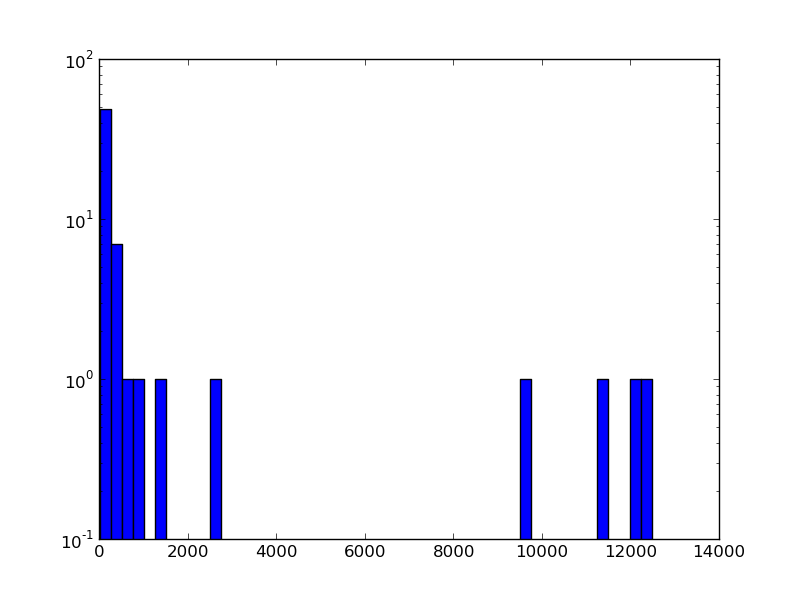
\includegraphics[scale=.4]{networkx_community_dist.png} 
\caption{Community Size Distribution of projected graph using Louvain Method}
\label{fig:networkx_community_dist}
\endminipage\hfill
\minipage{0.49\textwidth}
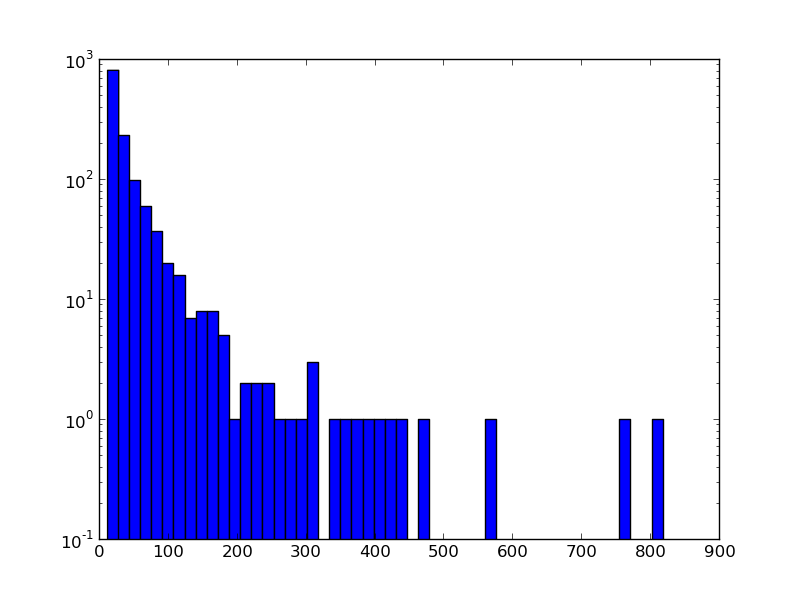
\includegraphics[scale=.4]{copra_community_dist.png}
\caption{Community Size Distribution of projected graph using label propogation}
\label{fig:copra_community_dist}
\endminipage\hfill
\end{figure}

\begin{figure}[ht]
\minipage{0.49\textwidth}
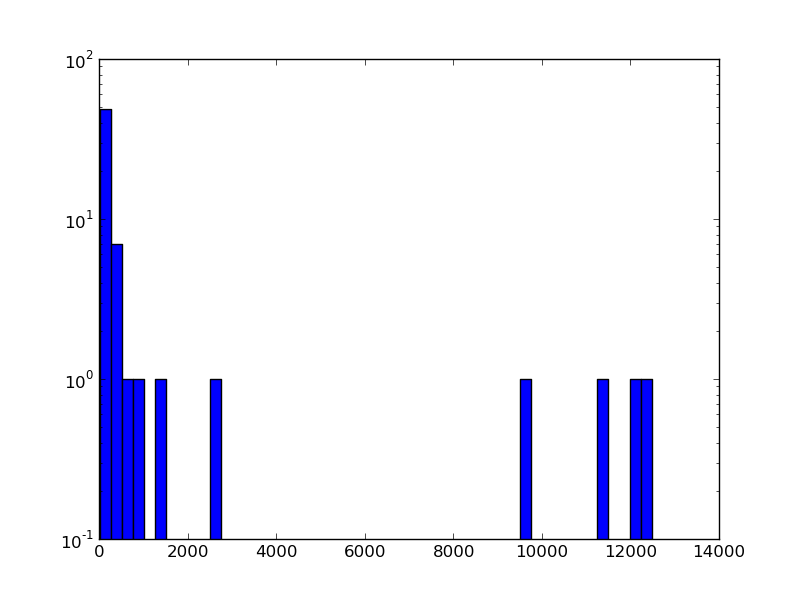
\includegraphics[scale=.4]{social_community_dist.png} 
\caption{Community Size Distribution of social graph using Louvain Method}
\label{fig:social_community_dist}
\endminipage\hfill
\end{figure}



\subsection{User Credibility}
\label{sec:user_credibility}

TODO Leyuan

\section{Results}
\label{sec:results}

To calculate a new business rating, we have three sets of people to pull information from: those inside our bipartite network community, those outside our bipartite network community, and those inside our social network community.  The weights of each group of users can be weighted differently.  We decided to test all different permuations of weights to see which one optimized the results the most.  For a certain weight permutation, we compute a new business score using Eq.\ref{avg_peer_value}.  For our results, we calculate this new business score for every user and every business and calculate the difference between what the user actually rated the business and what our new score is.  We imposed some size restrictions, such as forcing users to be in communities of at least 10 users or more.  The results for both community detection methods are shown in Figures \ref{fig:louvain_results} and \ref{fig:label_prop_results}.

\begin{multline}
\label{avg_peer_value}
NewScore(U, B) = peer\_rating(U, B)*peer\_weight + outsider\_rating(U, B)*outsider\_weight + \\
social\_rating(U, B) * social\_weight \\
\end{multline}

From the data, it's clear that our method is consistently worse than both Yelp and the HITS method.  The X axis is an index of a certain permutation.  A weight permutation of (0,0,1.0) would have an index of 0, while a permutation of (.1,0,.9) would have the index 11.  The Y axis is the mean difference between what a user rated a business and what we calculate that business score to be. The red 'Yelp' line is the difference to Yelp's standard rounded half-star rating; the yellow 'HITS' line is the difference to the HITS business score in Section \ref{sec:user_credibility}; the blue line is our diff using community detection.

Our best results occurred when peer\_weight=0.2, outsider\_weight=0.8, and social\_weight=0.0 for both detection methods, which is permutation index 21.

\begin{figure}[ht]
  \centering
    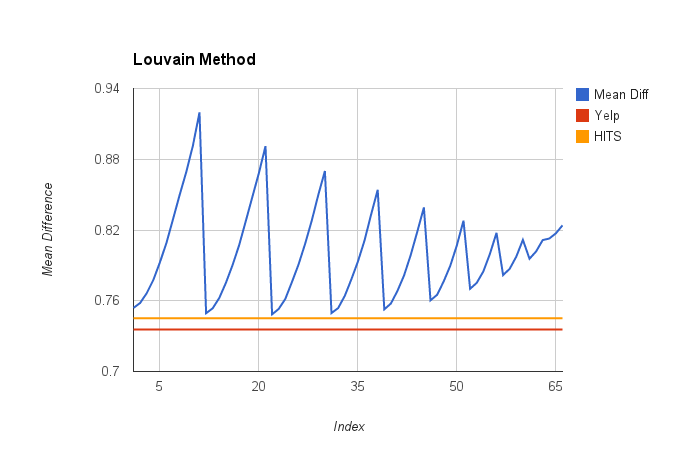
\includegraphics[width=0.75\textwidth]{louvain_results.png}
  \caption{Mean difference between Louvain method and actual ratings}
  \label{fig:louvain_results}
\end{figure}

\begin{figure}[ht]
  \centering
    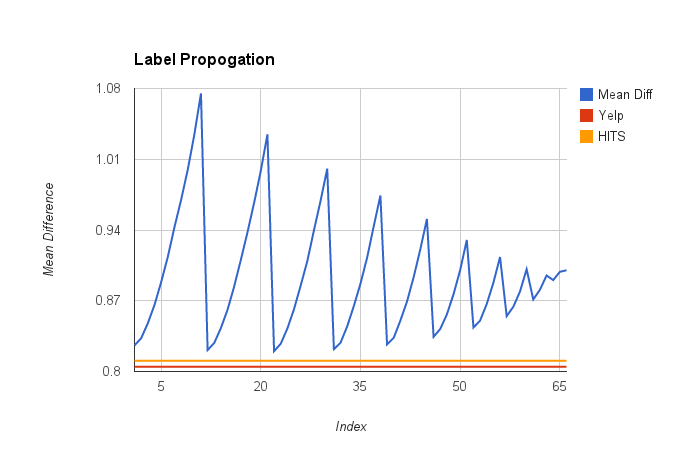
\includegraphics[width=0.75\textwidth]{label_prop_results.png}
  \caption{Mean difference between label propogation method and actual ratings (lower is better)}
  \label{fig:label_prop_results}
\end{figure}

\section{Conclusion}
\label{sec:conclusion}

It's unfortunate that our results were not very good, and there are many things that could be improved on.  For one, because of our reliance on networkx and python, we were quite computationally limited.  This meant we were working with an incomplete set of data.  If we had more computation power or wrote our code more efficiently, it would've been amazing to see how all of our tunable paramaters changes the final mean difference.  Things like our Jaccard threshold, min community size, min number of friends, min number of reviews, etc.  From our proposal, we really wanted to see if there was some phase transition when our method would suddenly become more effective once a user hit a sweet spot of friends/reviews - unfortunately we had neither the time nor coding skills to implement this efficiently.

We would've loved to do more community detection algorithms and see what difference that would've made.  We did not fully understand the clustering algorithms we were doing, and some of the attributes like weights and overlapping communities weren't utilized to its fullest.

While there are many improvements on the technical side, if we take our results at fact value, we can still come to an interesting conclusion.  From the data, it would seem that your friends or those people who review similar restaurants as you are no better predictors of your rating than the general population.  In fact, as we start including more and more weight to peer\_weight than outsider\_weight (which can be seen as the minimum peeks in the difference graphs), we slowly increase.  In other words, the general concensus on a restaurant tends to be a more accurate predictor for any user simply because of larger sample size.


Code for this project can be viewed at \url{https://github.com/edmundyan/yelp}

\printbibliography

\end{document}
